\chapter{Body-worn Sensor Technology}
The purpose of this chapter is to give an insight into relevant commercial products that exist today. It starts off by looking at the communities that surround these products before presenting the technology itself. Finally we discuss and display how these products present their activity data.

\section{Personal Informatics and Quantified Self}
Currently there are two names that stand out within the self-monitoring field: \gls{qs} \cite{quantifiedSelf}, and Personal Informatics (PI) \cite{personalInformatics}. \gls{qs} is a community of end-users who share data and exchange experiences with tools that help them collect information. \gls{pi} is a label used to classify a set of tools used for self monitoring. \gls{pi} also refers to a community that hosts conferences concerning research in the field of \gls{pi}.

\subsection{Personal Informatics}
Personal informatics is the label used to classify tools that help people collect personal information for the purpose of self-monitoring and self reflection. These tools are used to help individuals gain self-knowledge about their behaviour, habits, and thoughts.

The \gls{chi} conference has since 2010 \cite{chi2010} held workshops and accepted papers on Personal Informatics. The aim is to increase the understanding of how the tools affect the users as well as explore new possibilities, and overall improvement of the user experience.

\subsection{Quantified Self}
In 2011 \gls{qs} had their first conference \cite{bodyHackers}. Here people shared data that they had collected about themselves using different types of devices. Members of the community collect information about everything from sleep patterns and diets to mood and stress levels. The goal is to use quantitative data to improve ones own life, either through a more healthy lifestyle or by achieving a better understanding of oneself. 

To promote further development in tools that gather these types of information, the participants of Quantified Self have worked closely with companies and individuals that create personal informatics tools. Devices such as Nike's FuelBand and Fitbit are results of this cooperation, and both products have been well received by the community.

\section{Sensor technology}
% REVIEW: Read and give your judgement.
This section covers some popular commercial activity monitoring sensors currently on the market. The products that will be discussed are Nike Fuelband, Fitbit Flex and activPAL. Both Nike FuelBand and Fitbit Flex are designed for the personal use, while activPAL is manly used in research projects.

\subsection{Wrist-worn body sensors}
Since the release of the Nike+ FuelBand~\cite{fuelBand} in early 2012 several new wrist-worn activity monitors have emerged. Nike FuelBand, Fitbit Flex~\cite{flex} and Jawbone Up~\cite{jawboneUp} are the only ones, so far, who are either available to the public or soon to be released. The devices are designed to be inconspicuous, durable and to quietly monitor the users activity by counting steps taken, kilometres walked, time spent sleeping or sedentary etc. All of the bracelets use a built in 3-axis accelerometer to record movement. The classification of activity level is done by individual proprietary algorithms for each of the products.

\begin{figure}[h!]
  \centering
  \begin{subfigure}[b]{0.3\textwidth}
    \centering
    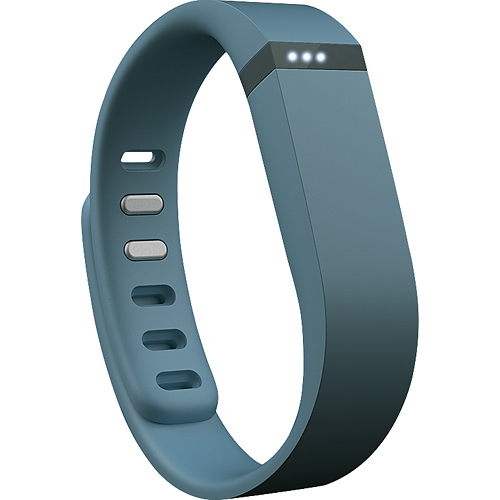
\includegraphics[width=\textwidth]{fitbitFlex.png}
    \caption{Fitbit Flex}
    \label{fig:fitbitFlex}
  \end{subfigure}
  \begin{subfigure}[b]{0.4\textwidth}
    \centering
    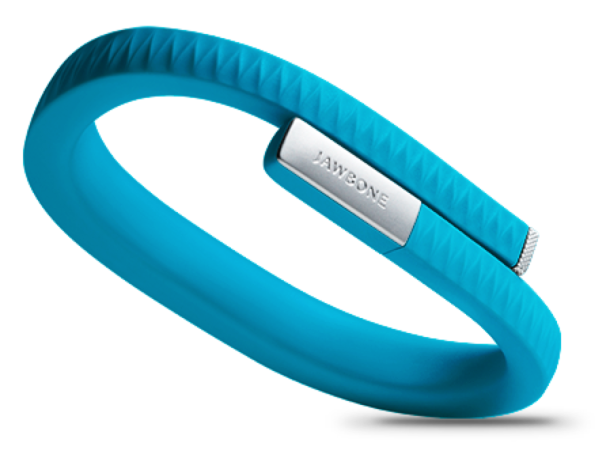
\includegraphics[width=\textwidth]{jawboneUp.png}
    \caption{Jawbone Up}
    \label{fig:jawboneUp}
  \end{subfigure}
  \caption[Fitbit Flex and Jawbone Up]{Two commercial wrist worn body sensors.}
\end{figure}

Being worn on the wrist these devices come with certain drawbacks, all the information gathering is based on movement from a single point (i.e. the users wrist). This leads to certain physical activities not being registered properly, one such example is riding a bike. The Fitbit developers have attempted to compensate for this by allowing the user to track such activity manually. The manually entered data is then added to the daily statistics. 

\subsection{activPAL}
\label{sensorActivPal}
The activPAL sensor has the shape of a small rectangle and is worn on the thigh. When the device is active it continuously records accelerometer data using an internal accelerometer. This data can be interpreted using algorithms provided by PAL Technologies.

\begin{figure}[h!]
	\centering
		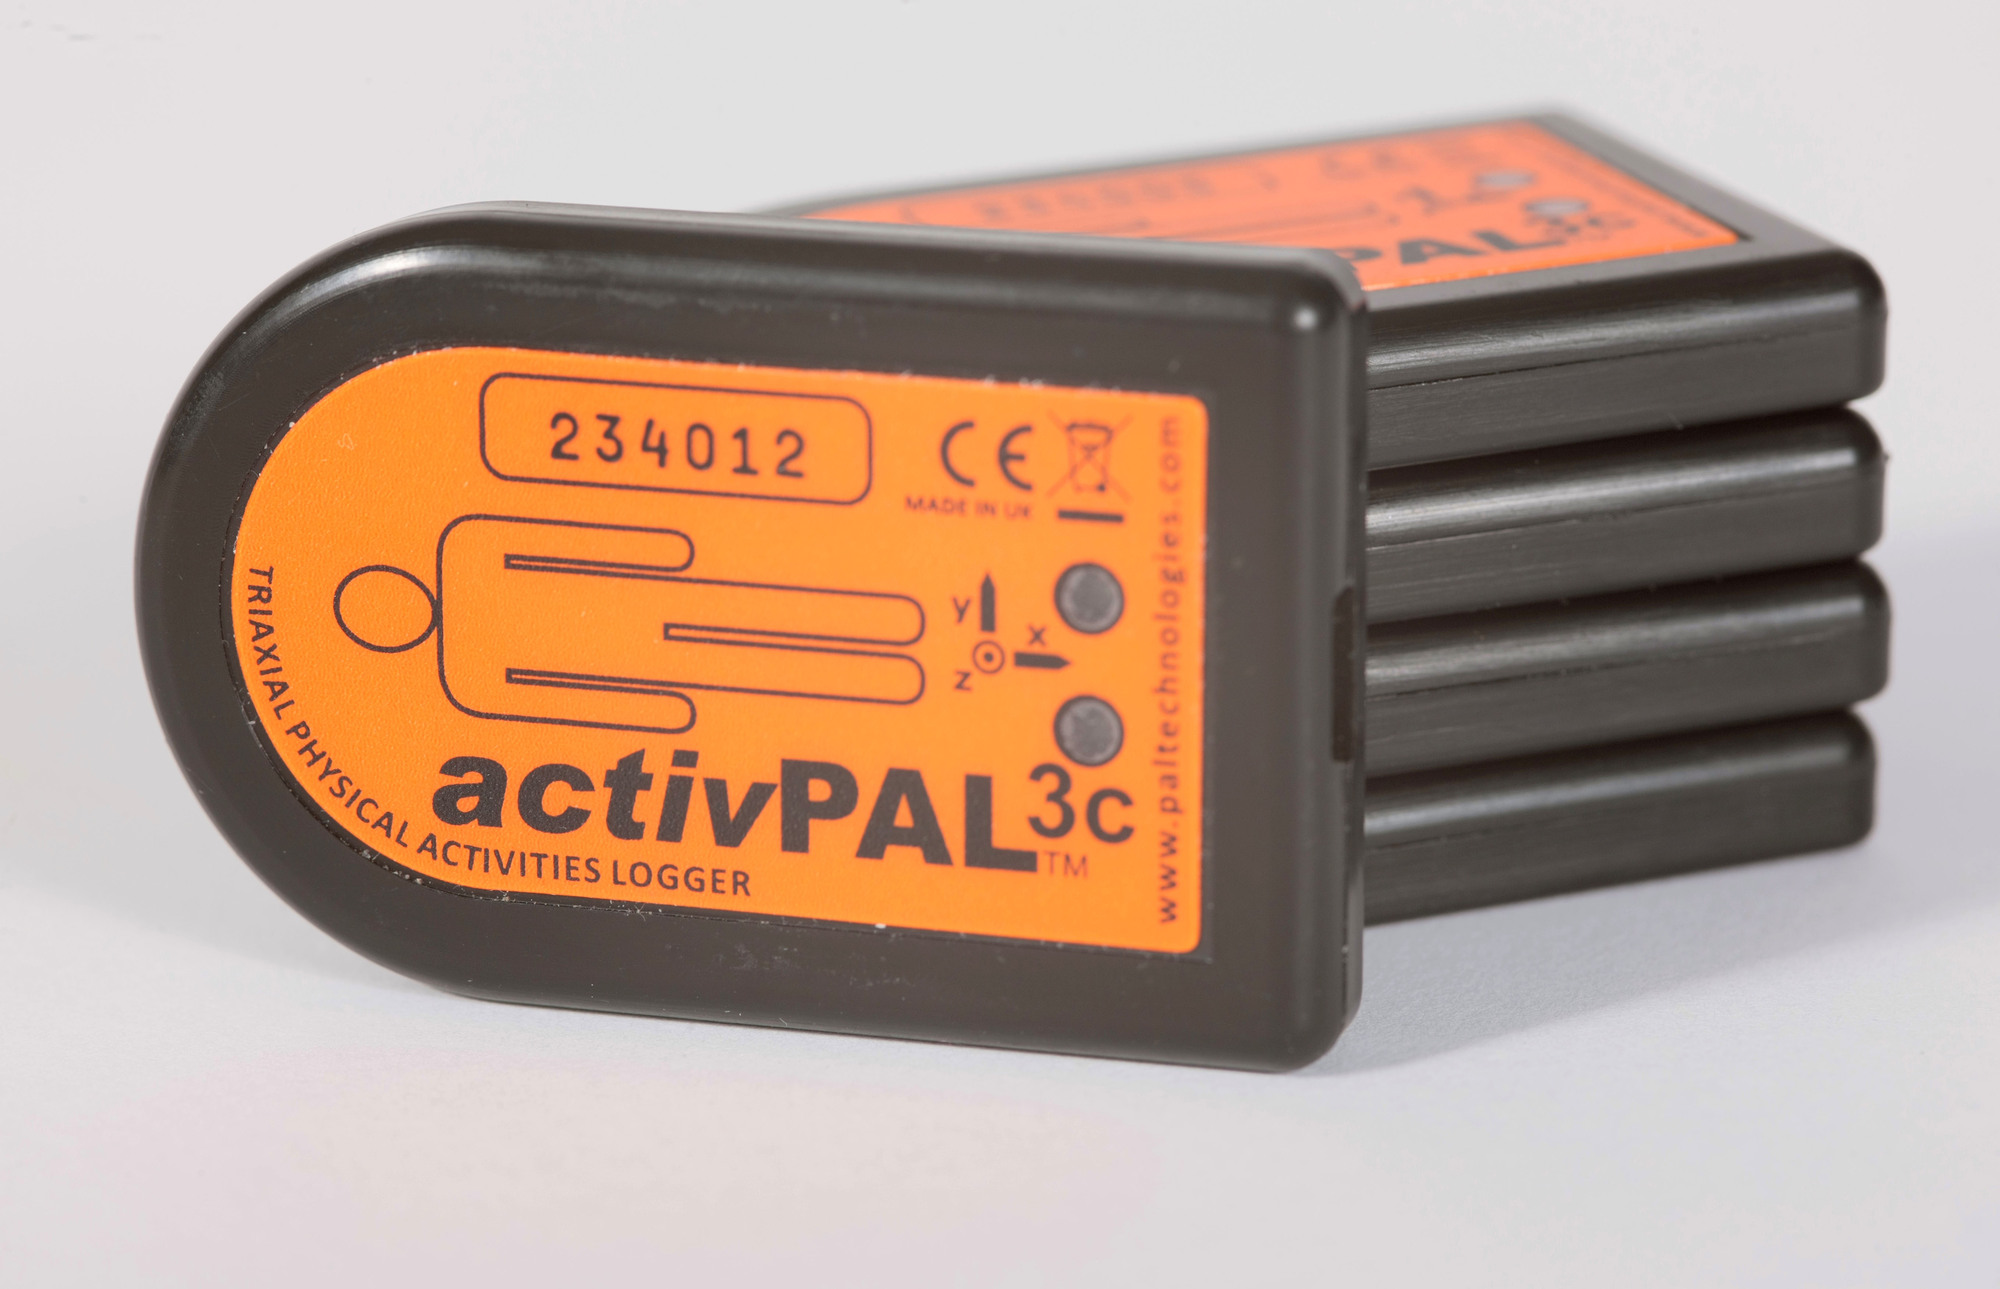
\includegraphics[width=0.6\textwidth]{activPALs.jpg}
		\caption[activPal sensor]{An activPAL tri-axis sensor.}
		\label{fig:activPal}
\end{figure}

When the activity data has been gathered the \emph{Intelligent Activity Classification}-algorithm is used to classify the data into three states: sitting/lying, standing and walking. Because activPAL is worn on the thigh, the accelerometer is unable to detect the difference between sitting and lying. Number of steps is also counted when walking.

% REVIEW ME and next section
activPAL differs from the other sensor presented in this chapter as it is designed for use in research and not commercial use. The sensor has a longer battery life than Fitbit Flex and Nike+ Fuelband, but does not include a practical way to be carried and has to be taped to the thigh. It is also much bigger than Fitbit Flex and Nike FuelBand. 

activPAL is frequently used in research, several studies have been conducted which conclude that the sensor is viable for recording and classifying activity \cite{grant2006, ryan2006, grant2008, tsavourelou}. The sensor has also been used in multiple studies for obtaining and analysing activity patterns~\cite{grant2010, lord, ryan2010}.

\section{Presentation of sensor data}
In this section we look at how the commercial activity monitoring devices presented in the previous section visualize their data. We will show that the Nike Fuelband and Fitbit Flex, designed for the general public, have a much broader range of visualizations with greater emphasis of being visually appealing than activPal.

\subsection{Nike+}
NikeFuel \cite{nikefuel} is a unit of measurement used by all Nike's activity trackers. The FuelBand does calculate steps and calories burned, but the NikeFuel is the prime focus of their product line. NikeFuel does not take into account gender, height, weight, but looks purely at activity. Meaning that a kilometer of walking will award the same amount of points to users with very different physiology. The daily progress (Figure \ref{fig:tworings}) is represented through a ring that fills up when the FuelBand detects activity. A full ring means that the daily goal has been reached. Progress beyond the daily goal will be displayed with numbers and visual enchantments on the ring. 


\begin{figure}[h!]
 \centering
  \begin{subfigure}[b]{0.49\textwidth}
    \centering
    \includegraphics[width=0.5\textwidth]{nikering.png}
    \caption{User having one third of his daily NikeFuel goal~\cite{fuelbandDcRain}.}
  \end{subfigure}
  \begin{subfigure}[b]{0.49\textwidth}
    \centering
    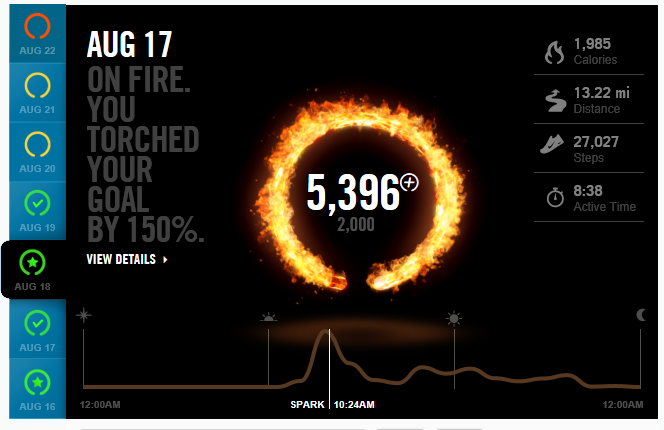
\includegraphics[width=\textwidth]{ringfire.png}
    \caption{User beating his daily limit by 150\%, rewarding him with special effects on the ring~\cite{fuelbandTechSpce}.}
  \end{subfigure} 
  \caption[Nike+ visualisations]{Two examples of Nike+ visualizations.}
  \label{fig:tworings}
\end{figure}

An online profile provides detailed information about the users activity, showing steps, calories burned, active time, distance travelled and average fuel, as seen in Figure~\ref{fig:activityBreakdown}. Charts can be displayed for weeks, months or years. This allows the user to track their progress and look at how often they achieve or exceed their goals~\cite{fuelbandTechSpce}. 

\begin{figure}[h!]
	\centering
		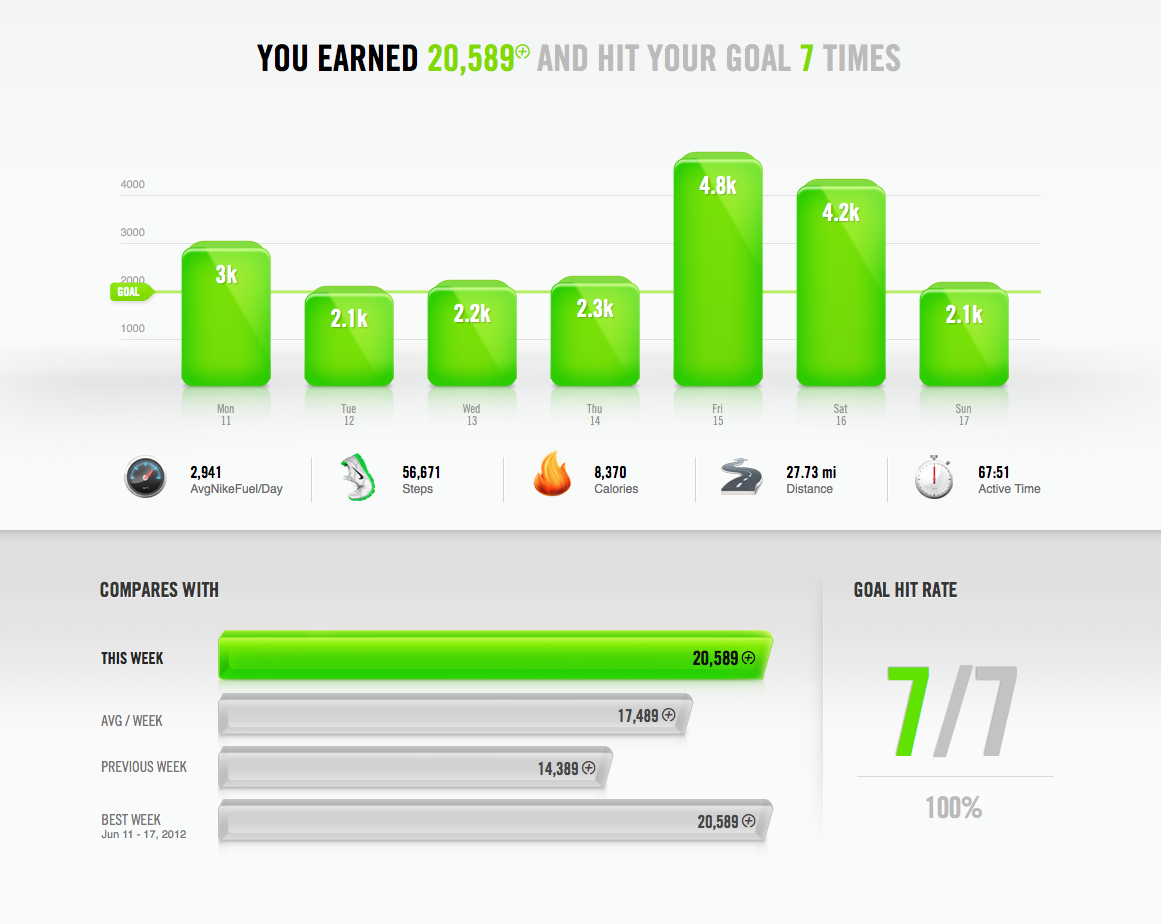
\includegraphics[width=0.7\textwidth]{week.png}
		\caption[Weekly breakdown (Nike)]{The weekly breakdown presented by Nike+. \cite{fuelbandTechSpce}}
		\label{fig:activityBreakdown}
\end{figure}

Virtual trophies are awarded for various achievements such as gathering an x amount of NikeFuel or beating the set goal by a 100\%. These trophies can then be shared with friends or displayed on the public profile to show off achievements. A review has reported that the NikeFuel concept can almost become an addiction and lead to doing some last minute workouts in order to reach the goal~\cite{fuelbandDcRain}.

\subsection{Fitbit}
Similar to the Nike+, Fitbit \cite{fitBit} allows the user to set daily goals, but as the Fitbit does not use the NikeFuel system. Instead it allows the user to set 3 separate goals: steps taken, floors climbed, and calories burned, as seen in Figure~\ref{fig:fitbitActivityBreakdown}. The Fitbit provide an active score, but there is no emphasis on it. On the Fitbit-webpage daily activity breakdown is provided. Activity levels are separated into four categories: sedentary, lightly active, fairly active, and very active. All the goal histories can be viewed on the online profile and can be categorized into day, week, months and years. 

Fitbit also offers the Fitbit Premium service, which adds more functionality to the online webapp. The premium service allows the user to get more detailed and aggregated information than the basic logs do. It gives advice on sleep, activity and food based on activity level and the recommended values for people in the users height, weight, age group.

\begin{figure}[h!]
	\centering
		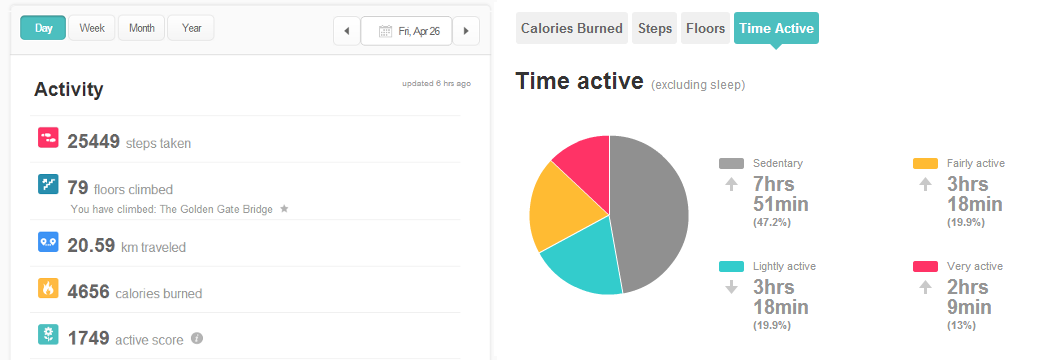
\includegraphics[width=0.9\textwidth]{fitbitActivityBreakdown.png}
		\caption[Fitbit+ visualizations]{The breakdown provided by FitBit. It can be broken into day, week, month, or year.}
		\label{fig:fitbitActivityBreakdown}
\end{figure}

\subsection{activPAL}
\label{sec:activPALViz}
The activPAL only provides one diagram, which can be seen in Figure~\ref{fig:activPalActivityBreakdown}. Yellow represents a sedentary position, green indicates an upright position and red means that the user was walking. If there is activity during an hour, the bar will rise and the activity will be colour coded to either red or green depending on their activity type. Looking at Figure~\ref{fig:activPalActivityBreakdown} we can see that at 10 AM the person spent a long time standing, a little while walking and almost no time was spent in a sedentary position. The pie chart and numbers to the right use the same colour coding and summarizes the activity distribution throughout the day.

\begin{figure}[h!]
	\centering
		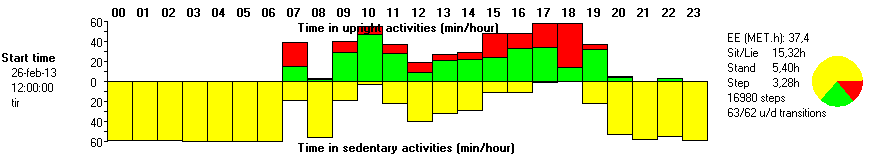
\includegraphics[width=1\textwidth]{activPalChart.png}
		\caption[activPal visualizations]{Visualization of sensor data from activPAL sensor.}
		\label{fig:activPalActivityBreakdown}
\end{figure}
